\chapter{IMPLEMENTASI}
	Bab ini membahas mengenai implementasi dari sistem yang sudah di desain dan dirancang pada bab sebelumnya. Pembahasan secara rinci akan dijelaskan pada setiap komponen yang ada yaitu load generator, pengambil data uji beban dan service controller yang meliputi web service, basis data dan task queue.
	
	\section{Lingkungan Implementasi}
		Dalam mengimplementasikan sistem pada tugas akhir ini, digunakan beberapa perangkat pendukung sebagai berikut.
		
		\subsection{Perangkat Keras}
		Perangkat keras yang digunakan dalam pengembangan sistem adalah sebagai berikut:
		\begin{enumerate}
			\item Web service dan task queue, processor AMD FX-7600P Radeon R7, 12 Compute Cores 4C+8G dan RAM 8GB.
			\item Node swarm dengan IP 167.71.194.235, processor Intel(R) Xeon(R) CPU E5-2650 v4@2.20GHz dan RAM 4GB.
			\item Node swarm dengan IP 165.22.55.82, processor Intel(R) Xeon(R) CPU E5-2650 v4@2.20GHz dan RAM 4GB.
			\item Node swarm dengan IP 167.71.194.233, processor Intel(R) Xeon(R) CPU E5-2650 v4@2.20GHz dan RAM 4GB.
			\item Basis data MySQL dengan IP 178.128.123.143, processor Intel(R) Xeon(R) Gold 6140 CPU@2.30GHz dan RAM 1GB.
		\end{enumerate}
	
		\subsection{Perangkat Lunak}
		Perangkat lunak yang digunakan dalam pengembangan sistem adalah sebagai berikut:
		\begin{enumerate}
			\item Sistem Operasi Ubuntu 18.04 LTS 64 Bit
			\item Docker versi 18.09.6 
			\item Headless Chrome 
			\item Puppeteer versi 0.12.0
			\item NPM versi 6.4.1
			\item Node.js versi 8.15.1
			\item Python versi 3.6.8
			\item MySQL Ver 14.14 Distrib 5.7.26
			\item Shell Script
			\item PHP dan Laravel 5.8
		\end{enumerate}
		
	\section{Implementasi Load Generator}
		Berdasarkan perancangan dan desain, load generator merupakan aktor yang akan berfungsi menggantikan pengguna ketika mengakses ke web. Load generator yang akan digunakan adalah Docker, namun diperlukan beberapa tahap untuk bisa menggunakan Docker atau kontainer sebagai load generator, yaitu tahap pemasangan dan konfigurasi. Tahap pemasangan docker dapat dilihat di Kode Sumber \ref{instalasidocker}, sedangkan untuk konfigurasi akan dibagi menjadi beberapa tahap yaitu:
		\begin{enumerate}
			\item Pembuatan Docker Image
			\item Pembuatan lingkungan kontainer
			\item Pemasangan Headless Chrome dan Puppeteer
		\end{enumerate}
			
		\subsection{Implementasi Pembuatan Docker Image}
			Docker Image digunakan untuk menjalankan kontainer, pada tugas akhir ini Docker Image akan dibuat terlebih dahulu agar bisa digunakan untuk menjalankan Puppeteer dan Headless Chrome. Namun untuk membuat Docker Image diperlukan beberapa tahapan yaitu konfigurasi Dockerfile, pemasangan Docker Compose dapat dilihat pada Kode Sumber \ref{dockercomposeinstall} dan konfigurasi docker-compsoe.yml dan unggah Docker Image ke Docker Hub.
			
			\indent Konfigurasi Dockerfile dapat dilihat pada Kode Sumber \ref{dockerimage}, sedangkan konfigurasi docker-compose.yml dapat dilihat pada Kode Sumber \ref{dockercompose}.
				\begin{lstlisting}[frame=single,tabsize=2,breaklines,caption={Konfigurasi Dockerfile },label=dockerimage, captionpos=b, language=json]
	FROM node:8
	RUN apt-get update
	# for https
	RUN apt-get install -yyq ca-certificates
	# install libraries
	RUN apt-get install -yyq libappindicator1 libasound2 libatk1.0-0 libc6 libcairo2 libcups2 libdbus-1-3 libexpat1 libfontconfig1 libgcc1 libgconf-2-4 libgdk-pixbuf2.0-0 libglib2.0-0 libgtk-3-0 libnspr4 libnss3 libpango-1.0-0 libpangocairo-1.0-0 libstdc++6 libx11-6 libx11-xcb1 libxcb1 libxcomposite1 libxcursor1 libxdamage1 libxext6 libxfixes3 libxi6 libxrandr2 libxrender1 libxss1 libxtst6
	# tools
	RUN apt-get install -yyq gconf-service lsb-release wget xdg-utils
	RUN apt-get install -yyq fonts-liberation 
	COPY code /app/code
	COPY output /app/output
	WORKDIR /app/code
	RUN yarn install
				\end{lstlisting}
				
				\begin{lstlisting}[frame=single,tabsize=2,breaklines,caption={Konfigurasi docker-compose.yml },label=dockercompose, captionpos=b, language=json]
	version: '3'
	services:
		puppeteer:
			build: .
			shm_size: '1gb'
			entrypoint: ["sh", "-c", "sleep infinity"]
				\end{lstlisting}
				
				Kemudian jalankan perintah Docker Compose berikut untuk pembuatan Docker Image.
				\begin{lstlisting}[frame=single,tabsize=2,breaklines,caption={Perintah untuk menjalankan  Docker Compose},label=createimg, captionpos=b, language=json,numbers=none]
	$ docker-compose up
				\end{lstlisting}
				
				Setelah Docker Image terbuat, ubah nama Docker Image tersebut dan melakukan commit agar bisa di push. Perintah pada kode sumber \ref{pushimagedocker} yang digunakan oleh penulis ketika mengunggah Docker Image ke Docker Hub.
				\begin{lstlisting}[frame=single,tabsize=2,breaklines,caption={Perintah untuk mengunggah Docker Image},label=pushimagedocker, captionpos=b, language=json,numbers=none]
	$ docker tag puppeteer_puppeteer:latest cphikmawan/ta2019:newpupp
	
	$ docker push cphikmawan/ta2019:newpupp
				\end{lstlisting}
				
		\subsection{Implementasi Pembuatan Lingkungan Kontainer}
			Kontainer akan dipasangkan pada suatu lingkungan yang bisa mengatur segala aktivitas kontainer, lingkungan yang akan dibangun pada sistem menggunakan alat orkestrasi yaitu Docker Swarm. Untuk mengimplementasikan Docker Swarm pada sistem ini, dibutuhkan satu node host sebagai manager node dan dua lainnya sebagai worker. Tahap pertama yang dilakukan yaitu menginisiasi salah satu node host yang akan digunakan sebagai manager node. Perintah inisiasi manager node terdapat pada Kode Sumber \ref{swarminit}.
			\begin{lstlisting}[frame=single,tabsize=2,breaklines,caption={Perintah untuk inisiasi manager node},label=swarminit, captionpos=b, language=json,numbers=none]
	$ docker swarm init --advertise-addr [IP NODE]
			\end{lstlisting}
			
			Setelah perintah pada kode sumber \ref{swarminit} dijalankan, maka manager node akan menghasilkan sebuah token yang digunakan oleh node host yang lain untuk bergabung sebagai worker. Perintah yang harus dijalankan pada setiap node host yang lain terdapat pada Kode Sumber \ref{swarmjoin}.
			\begin{lstlisting}[frame=single,tabsize=2,breaklines,caption={Perintah untuk bergabung ke Swarm},label=swarmjoin, captionpos=b, language=json,numbers=none]
	$ docker swarm join --token [token] [IP MANAGER]:2377
			\end{lstlisting}
			
			Tahap terakhir yang dilakukan yaitu memastikan semua node host sudah tergabung dengan manager node.
			\begin{lstlisting}[frame=single,tabsize=2,breaklines,caption={Perintah untuk melihat daftar Swarm Node},label=dockernodels, captionpos=b, language=json,numbers=none]
	$ docker node ls
			\end{lstlisting}
			
		\subsection{Implementasi Pemasangan Headless Chrome dan Puppeteer}
			Headless Chrome dan Puppeteer akan dipasang pada masing-masing kontainer menggunakan Docker Image yang telah dibuat sebelumnya, untuk pemasangannya akan dilakukan dilingkungan Docker Swarm dan dilakukan pada manager node. Namun untuk implementasinya dibutuhkan beberapa persiapan dan konfigurasi yang harus dilakukan terlebih dahulu yaitu konfigurasi unduh Docker Image, konfigurasi membuat Docker Network, konfigurasi puppeteer.yml, konfigurasi deployment.
			
			\indent Untuk mengunduh Docker Image dilakukan pada setiap node host menggunakan perintah pada Kode Sumber \ref{unduhimage} dan membuat Docker Network pada Kode Sumber \ref{createnetwork}. Sedangkan konfigurasi puppeteer.yml dapat dilihat di Kode Sumber \ref{puppyaml}
			\begin{lstlisting}[frame=single,tabsize=2,breaklines,caption={Perintah untuk mengunduh Docker Image },label=unduhimage, captionpos=b, language=json,numbers=none]
	$ docker image pull cphikmawan/ta2019:puppeteer
			\end{lstlisting}
			
			\begin{lstlisting}[frame=single,tabsize=2,breaklines,caption={Perintah untuk membuat Docker Network },label=createnetwork, captionpos=b, language=json,numbers=none]
	$ docker network create \
		--driver overlay \
		--subnet 10.0.0.0/18 \
		--attachable \
		[nama_network]
			\end{lstlisting}
			
			\begin{lstlisting}[frame=single,tabsize=2,breaklines,caption={Konfigurasi puppeteer.yml},label=puppyaml, captionpos=b, language=json]
	version: '3'
	# konfigurasi service
	services:
		# nama service yang akan dibuat
		puppeteer:
			# docker image yang digunakan
			image: cphikmawan/ta2019:newpupp
			# sinkronisasi penyimpanan antara kontainer dengan host
			volumes:
				- ./output:/app/output
				- ./code:/app/code
			# direktori kerja didalam kontainer
			working_dir: /app/code
			# konfigurasi untuk jumlah kontainer dan handling
			deploy:
				replicas: 1000
				restart_policy:
					condition: on-failure
			# entrypoint awal tidak akan melakukan apapun
			entrypoint: ["sh", "-c", "sleep infinity"]
	# konfigurasi jaringan
	networks:
		default:
			# jaringan default akan diubah ke jaringan eksternal
			external:
				# akan terkonek ke jaringan "swarm-network"
				name: swarm-network
			\end{lstlisting}
			
			\indent Tahap selanjutnya adalah konfigurasi deployment dengan menjalankan perintah yang ditunjukkan pada Kode Sumber \ref{pemasanganstack} di terminal manager node
			\begin{lstlisting}[frame=single,tabsize=2,breaklines,caption={Perintah untuk pemasangan kontainer },label=pemasanganstack, captionpos=b, language=json,numbers=none]
	$ docker stack deploy --compose-file=puppeteer.yml [nama_stack]
			\end{lstlisting}
	
	\section{Implementasi Pengambil Data Uji Beban}
		Pengambil Data Uji Beban akan dilakukan menggunakan sebuah pustaka Node yaitu Puppeteer. Pada saat dilakukan uji beban, Puppeteer akan mengambil data uji beban dari Headless Chrome menggunakan API dari Puppeteer secara otomatis. Beberapa data uji beban yang akan diambil yaitu:
		\begin{enumerate}
			\item Response End \\
				Atribut ini menunjukkan waktu setelah user menerima byte terakhir dari dokumen sebelum koneksi transportasi ditutup.
			\item DOM Content Loaded \\
				Atribut ini menunjukkan waktu setelah dokumen sudah diterima oleh user.
			\item Load Event End \\
				Atribut ini mengembalikan waktu ketika memuat dokumen selesai.
			\item CSS Tracing End \\
				Atribut ini menunjukkan waktu dari ekstraksi akhir file CSS dimuat.
			\item First Meaningfulpain \\
				Atribut ini adalah atribut khusus yang ada pada Chrome yang menunjukkan bahwa segala konten halaman yang dimuat sudah ditampilkan di layar. \\
		\end{enumerate}
	 
	 	\indent Selain data uji beban diatas, Puppeteer juga digunakan untuk mengambil sebuah tangkapan layar sesuai skenario yang dikirimkan oleh pengguna dan mengambil data saat terjadi kegagalan saat memuat assets yang tertulis pada console browser. Adapun pseudocode untuk melakukan pengambilan data uji beban dapat dilihat pada Kode Sumber \ref{pseudocodepupp}.
	 	
	 	\begin{lstlisting}[frame=single,tabsize=2,breaklines,caption={Pseudocode Puppeteer },label=pseudocodepupp, captionpos=b, language=json]
 	Variable Declaration
 	Data = Read Scenario File Configuration
 	
 	TESTPAGE FUNCTION:
 		CALL HELPERS FUNCTION:
 			GET Navigation Start
 		START Trace CSS Data
 		Trying to Accessing Website
 		END Trace CSS Data
 		CALL HELPERS FUNCTION:
 			GET Extracted Performance Data
 			GET Extracted CSS Tracing
 			RETURN Extracted Data
 	END TESTPAGE FUNCTION
 	
 	HELPERS FUNCTION:
 		GET Navigation Start
 			RETURN Navigation Start
 		Extracted Performance Data = Performance Data * 1000 - Navigation Start
 			RETURN Extracted Performance Data
 		Extracted CSS Tracing = CSS Tracing / 1000
 			RETURN Extracted CSS Tracing 
 	End Helpers Function
 	
 	MAIN FUNCTION:
 		START Headless Browser
 		GET Error Console
 			RETURN Data to Database
 		TRY:
 			CALL TESTPAGE FUNCTION(Data):
 				Get Data From TestPage -> Save Data Uji Beban
 			GET Page Screenshoot -> Save Screenshoot
 		CATCH ERROR:
 			GET Error
 			GET Page Screenshoot -> Save Screenshoot
 	END MAIN FUNCTION
	 	\end{lstlisting}
	
	\section{Implementasi Service Controller}
		Berdasarkan desain dan perancangan, service controller terdiri dari komponen web service, basis data dan task queue. Semua komponen tersebut akan diimplementasikan pada satu komputer milik penulis yang akan digunakan untuk web service dan penggunaan task queue, serta satu buah server untuk basis data MySQL.
		
		\subsection{Implementasi Web Service}
			Pada implementasi web service dibutuhkan beberapa persiapan lingkungan yang perlu dilakukan, urutannya meliputi langkah-langkah berikut:
			\begin{enumerate}
				\item Instalasi PHP
				\item Instalasi Composer
				\item Instalasi Laravel versi 5.8
				\item Instalasi MySQL
			\end{enumerate}
			
			\indent Web service akan menggunakan bahasa PHP dan kerangka kerja Laravel versi 5.8, sedangkan Composer berfungsi untuk memanajemen instalasi pustaka pada PHP dan untuk penyimpanan data yang digunakan pada sistem akan disimpan pada basis data MySQL. Web service berfungsi untuk memudahkan user melakukan uji beban pada suatu web. Tampilan antarmuka pengguna ditunjukkan pada Gambar \ref{gambarweb}.
			
			\begin{figure}[H]
				\centering
				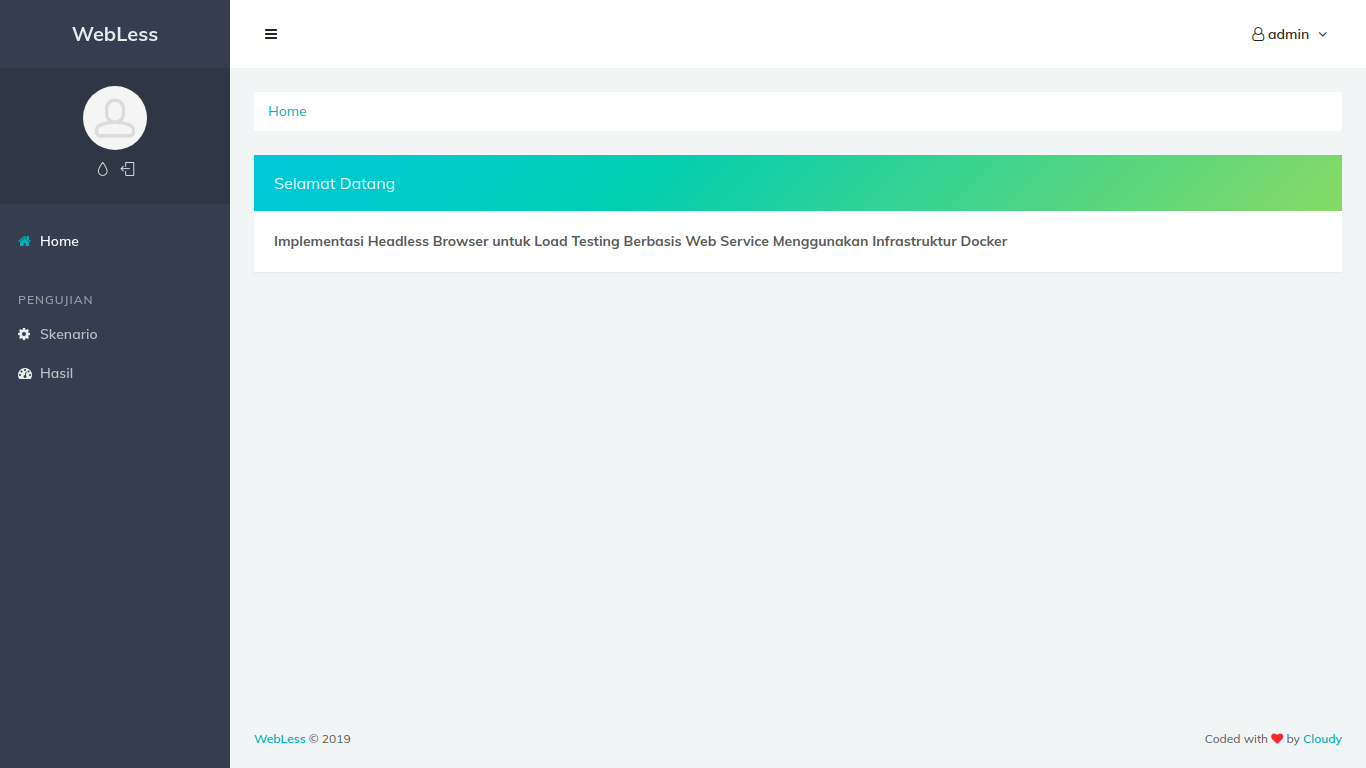
\includegraphics[width=10cm,height=6cm]{Images/C-4/gambarweb.png}
				\caption{Tampilan web antarmuka pengguna}
				\label{gambarweb}
			\end{figure}
			
			\indent Web service memiliki beberapa rute HTTP yang akan digunakan oleh user ketika mengakses web sistem. Rute-rute tersebut ditunjukkan pada Tabel \ref{tabelruteweb}.
			\begin{longtable}{|p{0.05\textwidth}|p{0.25\textwidth}|p{0.30\textwidth}|p{0.30\textwidth}|}
				\caption{Rute HTTP pada web service} \label{tabelruteweb} \\ \hline
				\textbf{No} & \textbf{Rute} & \textbf{Metode} & \textbf{Aksi} \\ \hline
				\endhead
				\endfoot
				\endlastfoot
				1 & / & GET & Mengakses halaman home \\ \hline
				2 & /login & GET & Mengakses halaman login \\ \hline
				3 & /login & POST & Melakukan login \\ \hline
				4 & /logout & GET & Melakukan logout \\ \hline
				5 & /skenario & GET & Melihat skenario \\ \hline
				6 & /skenario & POST & Menambahkan skenario \\ \hline
				7 & /skenario & DELETE & Menghapus skenario \\ \hline
				8 & /worker & GET & Mengakses halaman worker \\ \hline
				9 & /worker & POST & Menambahkan jumlah worker dan data antrian \\ \hline
				10 & /hasil/rata-rata & GET & Mendapatkan hasil pengujian \\ \hline
				11 & /hasil/error-console & GET & Mendapatkan error console web \\ \hline
				12 & /hasil/images & GET & Melihat tangkapan layar web \\ \hline
				13 & /antrian & GET & Melihat jumlah dan status antrian \\ \hline
				
			\end{longtable}
		
		\subsection{Implementasi Skema Basis Data}
			Berdasarkan hasil perancangan basis data pada bab sebelumnya. Data yang dibutuhkan dan digunakan oleh sistem akan disimpan di dalam basis data MySQL. Data yang disimpan adalah data node host swarm, data kontainer, data pengguna, data skenario pengujian, data antrian request, data hasil pengujian, data error console, data rata-rata hasil pengujian.
			
			\subsubsection{Tabel Swarms}
				Pada tabel swarms menyimpan data-data dari node host yang tergabung dilingkungan swarm. Berikut definisi tabel swarms pada Tabel \ref{tabelswarms}.
				
				\begin{longtable}{|p{0.05\textwidth}|p{0.30\textwidth}|p{0.20\textwidth}|p{0.35\textwidth}|}
					\caption{Tabel swarms} \label{tabelswarms} \\
					\hline
					\textbf{No} & \textbf{Kolom} & \textbf{Tipe} & \textbf{Keterangan} \\ \hline
					\endhead
					\endfoot
					\endlastfoot
					1 & id & bigint(20) & Sebagai primary key, nilai awal adalah auto\_increment. \\ \hline
					2 & swarm\_ip & varchar(255) & Menunjukkan IP dari node host \\ \hline
					3 & swarm\_username & varchar(255) & Menunjukkan username dari node host \\ \hline
					4 & swarm\_password & varchar(255) & Menunjukkan password dari node host \\ \hline
					5 & is\_used & smallint(6) & Menunjukkan status dari node host \\ \hline
				\end{longtable}
		
			\subsubsection{Tabel Containers}
				Padata tabel containers menyimpan data-data dari Docker Container yang akan digunakan sebagai load generator. Berikut definisi tabel containers pada Tabel \ref{tabelcontainers}.
				
				\begin{longtable}{|p{0.05\textwidth}|p{0.30\textwidth}|p{0.20\textwidth}|p{0.35\textwidth}|}
					\caption{Tabel containers} \label{tabelcontainers} \\
					\hline
					\textbf{No} & \textbf{Kolom} & \textbf{Tipe} & \textbf{Keterangan} \\ \hline
					\endhead
					\endfoot
					\endlastfoot
					1 & id & bigint(20) & Sebagai primary key, nilai awal adalah auto\_increment \\ \hline
					2 & task\_id & varchar(100) & Menunjukkan task id dari kontainer \\ \hline
					3 & node\_id & varchar(100) & Menunjukkan node id tempat kontainer dipasang \\ \hline
					4 & container\_id & varchar(100) & Menunjukkan id dari kontainer \\ \hline
					5 & node\_ip & varchar(100) & Menunjukkan IP tempat kontainer dipasang \\ \hline
					6 & node\_host & varchar(100) & Menunjukkan hostname tempat kontainer dipasang \\ \hline
					7 & status & smallint(6) & Menunjukkan flag status dari container \\ \hline
					8 & username & varchar(100) & Menunjukkan status kontainer yang sedang digunakan user \\ \hline
				\end{longtable}
		
			\subsubsection{Tabel Users}
				Pada tabel users menyimpan data-data pengguna web yang disediakan sistem. Berikut definisi tabel users pada Tabel \ref{tabelusers}. Data pengguna juga memiliki constraint dan disimpan pada Tabel role user \ref{tabelroleuser} dan Tabel roles \ref{tabelroles}.
				
				\begin{longtable}{|p{0.05\textwidth}|p{0.30\textwidth}|p{0.20\textwidth}|p{0.35\textwidth}|}
					\caption{Tabel users} \label{tabelusers} \\
					\hline
					\textbf{No} & \textbf{Kolom} & \textbf{Tipe} & \textbf{Keterangan} \\ \hline
					\endhead
					\endfoot
					\endlastfoot
					1 & id & bigint(20) & Sebagai primary key, nilai awal adalah auto\_increment \\ \hline
					2 & name & varchar(255) & Menunjukkan nama pengguna \\ \hline
					3 & email & varchar(255) & Menunjukkan email pengguna \\ \hline
					4 & username & varchar(255) & Menunjukkan username pengguna \\ \hline
					5 & password & varchar(255) & Menunjukkan password pengguna \\ \hline
				\end{longtable}
			
				\begin{longtable}{|p{0.05\textwidth}|p{0.30\textwidth}|p{0.20\textwidth}|p{0.35\textwidth}|}
					\caption{Tabel role user} \label{tabelroleuser} \\
					\hline
					\textbf{No} & \textbf{Kolom} & \textbf{Tipe} & \textbf{Keterangan} \\ \hline
					\endhead
					\endfoot
					\endlastfoot
					1 & id & bigint(20) & Sebagai primary key, nilai awal adalah auto\_increment \\ \hline
					2 & role\_id & int(10) & Menunjukkan id role pengguna \\ \hline
					3 & user\_id & int(10) & Menunjukkan id pengguna \\ \hline
				\end{longtable}
				
				\begin{longtable}{|p{0.05\textwidth}|p{0.30\textwidth}|p{0.20\textwidth}|p{0.35\textwidth}|}
					\caption{Tabel roles} \label{tabelroles} \\
					\hline
					\textbf{No} & \textbf{Kolom} & \textbf{Tipe} & \textbf{Keterangan} \\ \hline
					\endhead
					\endfoot
					\endlastfoot
					1 & id & bigint(20) & Sebagai primary key, nilai awal adalah auto\_increment \\ \hline
					2 & name & varchar(255) & Menunjukkan nama role \\ \hline
					3 & description & varchar(255) & Menunjukkan deskripsi hak akses dari nama role \\ \hline
				\end{longtable}
		
			\subsubsection{Tabel Scenarios}
				Pada tabel scenarios menyimpan data-data skenario yang telah dibuat oleh pengguna. Berikut definisi tabel scenarios pada Tabel \ref{tabelscenarios}.
			
				\begin{longtable}{|p{0.05\textwidth}|p{0.30\textwidth}|p{0.20\textwidth}|p{0.35\textwidth}|}
					\caption{Tabel scenarios} \label{tabelscenarios} \\
					\hline
					\textbf{No} & \textbf{Kolom} & \textbf{Tipe} & \textbf{Keterangan} \\ \hline
					\endhead
					\endfoot
					\endlastfoot
					1 & id & bigint(20) & Sebagai primary key, nilai awal adalah auto\_increment \\ \hline
					2 & scenario\_id & varchar(255) &  \\ \hline
					3 & username & varchar(255) &  \\ \hline
					4 & scenario\_method & varchar(255) &  \\ \hline
					5 & scenario\_link & varchar(255) &  \\ \hline
					6 & scenario\_worker & varchar(255) &  \\ \hline
					7 & scenario\_status & smallint(6) &  \\ \hline
				\end{longtable}
		
			\subsubsection{Tabel Queues}
				Pada tabel queues menyimpan data-data antrian request yang dilakukan oleh semua pengguna. Berikut definisi tabel queues pada Tabel \ref{tabelqueues}.
			
				\begin{longtable}{|p{0.05\textwidth}|p{0.30\textwidth}|p{0.20\textwidth}|p{0.35\textwidth}|}
					\caption{Tabel queues} \label{tabelqueues} \\
					\hline
					\textbf{No} & \textbf{Kolom} & \textbf{Tipe} & \textbf{Keterangan} \\ \hline
					\endhead
					\endfoot
					\endlastfoot
					1 & id & bigint(20) & Sebagai primary key, nilai awal adalah auto\_increment \\ \hline
					2 & created\_at & timestamp & Menunjukkan waktu pembuatan queue request oleh pengguna \\ \hline
					3 & username & varchar(255) & Menunjukkan keterangan pengguna pembuat request \\ \hline
					4 & worker & int(11) & Menunjukkan jumlah request yang diinginkan pengguna \\ \hline
					5 & status & smallint(6) & Menunjukkan status dari queue, nilai awal adalah 0 \\ \hline
				\end{longtable}
		
			\subsubsection{Tabel Results}
				Pada tabel results menyimpan data-data hasil uji beban yang dilakukan oleh kontainer dan puppeteer. Berikut definisi tabel results pada Tabel \ref{tabelresults}.
				
				\begin{longtable}{|p{0.05\textwidth}|p{0.30\textwidth}|p{0.20\textwidth}|p{0.35\textwidth}|}
					\caption{Tabel results} \label{tabelresults} \\
					\hline
					\textbf{No} & \textbf{Kolom} & \textbf{Tipe} & \textbf{Keterangan} \\ \hline
					\endhead
					\endfoot
					\endlastfoot
					1 & id & bigint(20) & Sebagai primary key, nilai awal adalah auto\_increment \\ \hline
					2 & scenario\_id & varchar(255) & Menunjukkan skenario id sebagai foreign key \\ \hline
					3 & link & varchar(255) & Menunjukkan link website yang diuji \\ \hline
					4 & method & varchar(100) & Menunjukkan metode uji \\ \hline
					5 & worker & varchar(255) & Menunjukkan jumlah request yang diinginkan pengguna \\ \hline
					6 & username & varchar(100) & Menunjukkan keterangan pengguna pembuat request \\ \hline
					7 & host & varchar(100) & Menunjukkan IP node host yang digunakan kontainer penguji \\ \hline
					8 & response\_end & varchar(100) & Menunjukkan hasil uji response time dalam satuan detik \\ \hline
					9 & dom\_content\_load & varchar(100) & Menunjukkan hasil uji waktu memuat DOM web dalam satuan detik \\ \hline
					10 & load\_event\_end & varchar(100) & Menunjukkan hasil uji load time dalam satuan detik \\ \hline
					11 & css\_trace\_end & varchar(100) & Menunjukkan hasil uji waktu memuat css time dalam satuan detik \\ \hline
					12 & first\_meaningful & varchar(100) & Menunjukkan hasil uji waktu memuat konten utama dalam satuan detik \\ \hline
					13 & status & smallint(6) & Menunjukkan status apakah untuk proses rata-rata, nilai awal adalah 0 \\ \hline
				\end{longtable}
		
			\subsubsection{Tabel Errors}
				Pada tabel errors menyimpan data-data kegagalan yang terekam pada console browser ketika diakses didalam Headless Chrome. Berikut definisi tabel errors pada Tabel \ref{tabelerrors}.
				
				\begin{longtable}{|p{0.05\textwidth}|p{0.30\textwidth}|p{0.20\textwidth}|p{0.35\textwidth}|}
					\caption{Tabel errors} \label{tabelerrors} \\
					\hline
					\textbf{No} & \textbf{Kolom} & \textbf{Tipe} & \textbf{Keterangan} \\ \hline
					\endhead
					\endfoot
					\endlastfoot
					1 & id & bigint(20) & Sebagai primary key, nilai awal adalah auto\_increment \\ \hline
					2 & scenario\_id & varchar(255) & Menunjukkan skenario id sebagai foreign key \\ \hline
					3 & link & varchar(255) & Menunjukkan link website yang diuji \\ \hline
					4 & worker & varchar(255) & Menunjukkan jumlah request yang diinginkan pengguna \\ \hline
					5 & username & varchar(100) & Menunjukkan keterangan pengguna pembuat request \\ \hline
					6 & host & varchar(100) & Menunjukkan IP node host yang digunakan kontainer penguji \\ \hline
					7 & type & varchar(100) & Menunjukkan type error \\ \hline
					8 & text & varchar(255) & Menunjukkan keterangan error \\ \hline
					9 & args & varchar(255) & Menunjukkan argumen error \\ \hline
					10 & location\_url & varchar(255) & Menunjukkan lokasi url error \\ \hline
				\end{longtable}
		
			\subsubsection{Tabel Summary Results}
				Pada tabel summary\_results menyimpan data rata-rata dari hasil uji beban yang ada pada tabel results. Berikut definisi tabel summary\_results pada Tabel \ref{tabelsumresults}.
			
				\begin{longtable}{|p{0.05\textwidth}|p{0.30\textwidth}|p{0.20\textwidth}|p{0.35\textwidth}|}
					\caption{Tabel summary results} \label{tabelsumresults} \\
					\hline
					\textbf{No} & \textbf{Kolom} & \textbf{Tipe} & \textbf{Keterangan} \\ \hline
					\endhead
					\endfoot
					\endlastfoot
					1 & id & bigint(20) & Sebagai primary key, nilai awal adalah auto\_increment \\ \hline
					2 & scenario\_id & varchar(255) & Menunjukkan skenario id sebagai foreign key \\ \hline
					3 & link & varchar(255) & Menunjukkan link website yang diuji \\ \hline
					4 & method & varchar(100) & Menunjukkan metode uji \\ \hline
					5 & worker & varchar(255) & Menunjukkan jumlah request yang diinginkan pengguna \\ \hline
					6 & username & varchar(100) & Menunjukkan keterangan pengguna pembuat request \\ \hline
					7 & error & varchar(100) & Menunjukkan presentase kegagalan saat dilakukan uji beban \\ \hline
					8 & response\_end & varchar(100) & Menunjukkan rata-rata hasil uji response time dalam satuan detik \\ \hline
					9 & dom\_content\_load & varchar(100) & Menunjukkan rata-rata hasil uji waktu memuat DOM web dalam satuan detik \\ \hline
					10 & load\_event\_end & varchar(100) & Menunjukkan rata-rata hasil uji load time dalam satuan detik \\ \hline
					11 & css\_trace\_end & varchar(100) & Menunjukkan rata-rata hasil uji waktu memuat css time dalam satuan detik \\ \hline
					12 & first\_meaningful & varchar(100) & Menunjukkan rata-rata hasil uji waktu memuat konten utama dalam satuan detik \\ \hline
				\end{longtable}
			
		\subsection{Implementasi Task Queue}
			Task queue akan digunakan untuk mengatur antrian request dari pengguna, pada tugas akhir ini implementasi task queue akan dipasang pada komputer yang sama dengan web service. Bahasa pemrograman yang akan digunakan untuk mengimplementasikan task queue adalah bahasa pemrograman Python, sedangkan untuk basis data akan terkoneksi dengan basis data MySQL yang terpasang pada server yang berbeda. Selain itu task queue akan dijalankan setiap 1 menit sekali pada crontab. Selama task queue berjalan algoritmenya akan selalu melakukan pengecekan apakah ada antrian yang bisa dieksekusi. Pseudocode untuk task queue tertera pada Kode Sumber \ref{taskqueue} dan untuk konfigurasi crontab pada Kode Sumber \ref{crontab}.
			
			\begin{lstlisting}[frame=single,tabsize=2,breaklines,caption={Konfigurasi docker-compose.yml },label=taskqueue, captionpos=b, language=json]
	Connection
	
	Variable Declaration

	DECLARE ADDITIONAL FUNCTION
		Get Data Task Queue from MySQL <- LIMIT 1
		RETURN data
	
	MAIN FUNCTION
		Data = CALL ADDITIONAL FUNCTION
		IF Data Not NULL
			Do Task Queue Job
		Else
		 RETURN Null to Output File
	END FUNCTION
			\end{lstlisting}
			
			\begin{lstlisting}[frame=single,tabsize=2,breaklines,caption={Konfigurasi docker-compose.yml },label=crontab, captionpos=b, language=json]
	* * * * * /usr/bin/python3 queue.py >> output.log 2>&1
			\end{lstlisting}